% =============================================================================
% NL2Semantic2SQL: Semantic Grounding and Safe Execution for PostGIS-based
% NL2GeoSQL, with a Cross-Domain Stress Test on Warehouse Queries.
% IJGIS double-anonymised submission.
% =============================================================================
\documentclass[11pt]{article}

\usepackage[margin=1in]{geometry}
\usepackage{times}
\usepackage{amsmath,amssymb}
\usepackage{graphicx}
\usepackage{booktabs}
\usepackage{multirow}
\usepackage{caption}
\usepackage{subcaption}
\usepackage{enumitem}
\usepackage{url}
\usepackage[hidelinks]{hyperref}
\usepackage{tikz}
\usetikzlibrary{positioning,arrows.meta,shapes.geometric,fit,calc}
\usepackage{algorithm}
\usepackage{algorithmic}

\title{Semantic Grounding and Safe Execution for PostGIS Natural-Language-to-SQL}
\author{Anonymous Author(s)\\ \textit{Affiliation withheld for double-anonymised review}}
\date{}

\begin{document}
\maketitle

% =============================================================================
\begin{abstract}
% =============================================================================
Natural language interfaces to geospatial databases must handle challenges that mainstream text-to-SQL benchmarks rarely exercise: geometry-aware schema grounding, OGC/PostGIS topological and metric predicates, coordinate reference systems, \texttt{::geography} casting, KNN operators, and safety-critical refusal of destructive or unbounded queries. We present \textbf{NL2Semantic2SQL}, a semantic-grounding and safe-execution framework for executable PostGIS NL2GeoSQL. It couples a semantic layer (aliases, geometry types, SRIDs, spatial operator rules) with an intent-conditioned router, schema-aware prompting, few-shot retrieval, a SQL postprocessor that enforces read-only safety and injects \texttt{LIMIT} on large-table preview queries, and an execution-time self-correction loop. The same bilingual architecture serves Chinese GIS and English warehouse queries from a single pipeline; we evaluate both sides so that the current state of each is measurable. We evaluate on a 125-question Chongqing PostGIS benchmark (85 Spatial + 40 Robustness across six safety categories) and on a warehouse evaluation track on BIRD mini\_dev, reported as a 108-question design set and a disjoint 150-question held-out set. On GIS Spatial we pool three independent Full-mode runs (each 85 questions) and report mean~$\pm$~SD EX$=0.663 \pm 0.048$ (range $[0.612, 0.706]$) vs.\ baseline $0.529$; the majority-vote Full result is $0.659$, with paired McNemar $p=0.052$ (marginal). Two of three individual samples reach significance ($p=0.003$, $p=0.029$); one does not. The 40-question Robustness suite is the strongest primary claim: Full reaches $39/40 = 0.975$ vs.\ baseline $0.450$ (paired McNemar $b=0$, $c=21$, $p<10^{-4}$), with OOM Prevention bounded-answer compliance improving from $1/8$ to $7/8$ after the \texttt{EXPLAIN}-based pre-check and a revised bounded-output agent prompt. On BIRD, the pipeline improves the design set by $+0.093$ ($p=0.0213$) but only $+0.033$ on the held-out set ($p=0.3833$, 95\% CI $[-0.03, 0.09]$); this current-state snapshot motivates a planned second round of warehouse-side grounding. A 50-question Chinese BIRD probe is additionally reported alongside a bilingual human re-audit (18~\textsc{ok}, 32~\textsc{fix}, 0~\textsc{drop}; post-review EX $0.540$ vs.\ pre-review $0.560$, paired $p=1.00$) that rules out translation artefacts as the cause of the English$\to$Chinese gap.
\end{abstract}

\noindent\textbf{Keywords:} NL2GeoSQL; PostGIS; natural language interface; geospatial database; semantic layer; spatial predicates; coordinate reference systems; safe execution; large language model.

% =============================================================================
\section{Introduction}
\label{sec:intro}
% =============================================================================

Natural language access to spatial databases is a long-standing GIScience problem~\cite{goodchild1992gis,egenhofer1991topological,clementini1993small}. Recent large language models have pushed general text-to-SQL forward on benchmarks such as Spider~\cite{yu2018spider} and BIRD~\cite{li2023bird}, yet these benchmarks deliberately abstract away the execution machinery that defines geospatial querying: the OGC Simple Feature Access predicates~\cite{ogcsfs}, coordinate reference system transformations, the \texttt{geometry}/\texttt{geography} type distinction, spatial indexes, KNN operators, and the safety constraints that any production GIS must enforce against destructive or unbounded queries. Natural language to executable PostGIS~\cite{postgis} (NL2GeoSQL) is therefore not an instance of text-to-SQL with a GIS dataset but a distinct problem shaped by spatial-database semantics.

The grounding stage is where the gap is most visible. General text-to-SQL schema linking aligns user expressions with column names; PostGIS grounding must additionally recognise geometry-bearing attributes, infer whether a question requires a topological predicate (\texttt{ST\_Intersects}, \texttt{ST\_Touches}, \texttt{ST\_Contains}), a metric operator (\texttt{ST\_Distance}, \texttt{ST\_DWithin}, \texttt{ST\_Area}), a buffer or KNN operator (\texttt{<->}), and decide when a geography cast or \texttt{ST\_Transform} is required so that area and distance are returned in metres rather than degrees. It must also refuse destructive intent (\texttt{DELETE}, \texttt{UPDATE}, \texttt{DROP}) and enforce bounded output on large-table preview queries. These are GIScience computations, not prompt-engineering problems.

We present \textbf{NL2Semantic2SQL}, a semantic-grounding and safe-execution framework for PostGIS-based NL2GeoSQL. A semantic layer provides aliases, geometry metadata, spatial operator rules, and safety constraints; a bilingual intent classifier routes Chinese GIS and English warehouse queries into the appropriate grounding path; a SQL postprocessor enforces read-only safety, repairs identifier quoting, and injects \texttt{LIMIT} on large-table preview queries; and an execution-time self-correction loop recovers from common PostGIS execution errors such as missing geography casts and mixed-case identifier quoting. The same framework serves both GIS and warehouse users, and we evaluate both sides so that the current state of each is measurable.

For primary evaluation, we construct a 125-question Chongqing PostGIS benchmark with executable gold SQL (85 Spatial covering OGC-Simple-Feature predicates, metric and KNN operators, CRS transforms, and aggregation across three difficulty levels; plus 40 Robustness spanning six safety and refusal categories). For the warehouse evaluation track, we use BIRD mini\_dev with a deliberate design/held-out split: a 108-question \emph{design set} used to derive grounding rules by error attribution, and a disjoint 150-question \emph{held-out set} for independent significance. We additionally run a 50-question cross-lingual probe on LLM-translated Chinese BIRD questions together with a bilingual human re-audit and paired re-run on the reviewed subset, so that translation-pipeline noise and genuine cross-lingual capability can be distinguished.

\medskip
\noindent\textbf{Contributions.} The principal contribution is PostGIS-side grounding; the BIRD evaluation is a second track that reports the current state of the warehouse path of the same framework.
\begin{enumerate}[leftmargin=*]
  \item \textbf{A semantic-grounding and safe-execution framework for NL2GeoSQL} that declares geometry types, SRIDs, spatial operator rules, and refusal constraints in a semantic layer and threads them through intent-conditioned routing, schema-aware prompting, SQL postprocessing, and execution-time self-correction.
  \item \textbf{A 125-question Chongqing PostGIS benchmark} with executable gold SQL verified against a live PostGIS database, explicitly separating 85 Spatial questions (OGC predicates, metric and KNN operators, CRS transforms, aggregation) from 40 Robustness questions (six safety categories). On GIS Spatial, three independent Full-mode runs yield pooled mean~$\pm$~SD EX$=0.663 \pm 0.048$ (range $[0.612, 0.706]$) vs.\ baseline $0.529$; two of three individual samples are paired-significant (paired McNemar $p=0.003$, $p=0.029$) and majority-vote $p=0.052$ (marginal). The 40-question Robustness suite is the strongest primary claim: Full reaches $39/40 = 0.975$ vs.\ baseline $18/40 = 0.450$ (paired McNemar $b=0$, $c=21$, $p<10^{-4}$), with OOM Prevention bounded-answer compliance reaching $7/8$ under the \texttt{EXPLAIN}-based pre-check and bounded-output agent prompt described in Section~\ref{sec:method}.
  \item \textbf{A warehouse evaluation track on BIRD mini\_dev} separating an 108-question design set (rule derivation) from a 150-question held-out set (independent significance). Grounding rules learned on the design set improve the design-set EX by $+0.093$ ($p=0.0213$) but improve held-out EX by only $+0.033$ (95\% CI $[-0.03, 0.09]$, $p=0.3833$), a current-state snapshot that we use to scope the next round of warehouse-side grounding work rather than a closed generalisation claim.
\end{enumerate}

The paper proceeds as follows. Section~\ref{sec:related} reviews GIScience foundations and the recent IJGIS-published NL-to-spatial-database literature. Section~\ref{sec:method} formalises the problem and details the architecture. Section~\ref{sec:experiments} presents the PostGIS evaluation and the BIRD warehouse evaluation track. Section~\ref{sec:discussion} discusses interpretation. Section~\ref{sec:conclusion} concludes.

% =============================================================================
\section{Related Work}
\label{sec:related}
% =============================================================================

\subsection{GIScience foundations for NL-to-spatial-database}

Natural language access to spatial databases sits within the GIScience programme articulated by Goodchild~\cite{goodchild1992gis}: formalising geographic concepts so they can be computed rigorously. The relational spatial semantics we ground against have roots in the $4$- and $9$-intersection formalisms~\cite{egenhofer1991topological} and the simplified end-user topological relations of Clementini et al.~\cite{clementini1993small} --- equals, disjoint, touches, contains, overlaps, within, crosses, intersects --- which the OGC Simple Feature Access standard codifies for relational spatial SQL~\cite{ogcsfs} and GeoSPARQL~\cite{ogcgeosparql} extends to RDF. PostGIS~\cite{postgis} operationalises these in PostgreSQL and defines the \texttt{geometry}/\texttt{geography} type distinction, the \texttt{::geography} cast, \texttt{ST\_DWithin}, \texttt{ST\_Transform}, and the \texttt{<->} KNN operator any PostGIS-generating system must respect. Our grounding rules encode these formalisms as prompt-side evidence.

\subsection{Natural language interfaces to spatial databases}

Early geospatial question answering focused on small fact databases: Zelle and Mooney~\cite{zelle1996geoquery} used inductive logic programming for GeoQuery, and Punjani et al.~\cite{punjani2018geospatial} extended this to template-based question answering over linked geospatial data, highlighting spatial-predicate coverage and coordinate-system awareness. Recent LLM-era work falls into two groups. The first targets end-to-end NL-to-executable-spatial-SQL: NALSpatial~\cite{liu2025nalspatial} translates user queries into spatial SQL over PostGIS-style backends; Monkuu~\cite{yu2025monkuu} is an IJGIS-published LLM-powered NL interface with dynamic schema mapping; GeoSQL-Eval~\cite{hou2026geosql} contributes the first large-scale LLM evaluation on PostGIS NL2GeoSQL (14{,}178 tasks across 340 PostGIS functions at function level). The second targets higher-level GeoAI agents: GeoCogent~\cite{houcoding2025} is an LLM-based agent for geospatial code generation; GeoAgent~\cite{lin2026geoagent} is a hierarchical multi-agent architecture. Surveys map the broader opportunities~\cite{mai2024foundation}. Our contribution lies at the narrower interface between spatial-database semantics and executable SQL: we study end-to-end execution-graded NL-to-PostGIS-SQL with a semantic-layer grounding that explicitly encodes OGC predicates, SRIDs, geography casts, and KNN operators, together with a postprocessor enforcing read-only and bounded-output semantics. Compared with NALSpatial and Monkuu we contribute a 125-question execution benchmark with an explicit Robustness suite, paired McNemar significance testing, and a design/held-out split on a warehouse benchmark as a second track of the same bilingual framework.

The comparison in Table~\ref{tab:related-comp} summarises capability and
evaluation practice across recent NL-to-spatial-database systems.

\begin{table}[t]\centering\footnotesize
\caption{Direct comparison to recent NL-to-spatial-database systems.
$\checkmark$: supported / reported; partial: some support; $-$: not reported.}
\label{tab:related-comp}
\begin{tabular}{@{}lcccccc@{}}
\toprule
System & Executable & Execution- & CRS / geog. & Safety / & Released & Paired \\
       & PostGIS    & based eval & / KNN       & refusal  & eval set & signif. \\
\midrule
NALSpatial~\cite{liu2025nalspatial}    & $\checkmark$ & $\checkmark$ & partial      & $-$           & $\checkmark$ & $-$           \\
Monkuu~\cite{yu2025monkuu}             & $\checkmark$ & $\checkmark$ & partial      & $-$           & $-$           & $-$           \\
GeoSQL-Eval~\cite{hou2026geosql}       & $-$           & $\checkmark$ & $\checkmark$ & $-$           & $\checkmark$ & $-$           \\
GeoCogent~\cite{houcoding2025}         & $-$           & $-$           & $-$           & $-$           & $-$           & $-$           \\
GeoAgent~\cite{lin2026geoagent}        & $-$           & partial      & partial      & $-$           & $-$           & $-$           \\
\textbf{Ours}                          & $\checkmark$ & $\checkmark$ & $\checkmark$ & $\checkmark$ & $\checkmark$ & $\checkmark$ \\
\bottomrule
\end{tabular}
\end{table}

\subsection{Text-to-SQL with LLMs and semantic layers}

LLM text-to-SQL has progressed through Spider~\cite{yu2018spider,rajkumar2022evaluating}, BIRD~\cite{li2023bird}, Spider~2.0~\cite{lei2025spider2}, and BEAVER~\cite{chen2024beaver}. DIN-SQL~\cite{pourreza2023dinsql} introduced decomposed in-context prompting with schema linking, query classification, generation, and self-correction; DAIL-SQL~\cite{gao2024dail} introduced skeleton-similarity few-shot selection; C3~\cite{dong2023c3} explored zero-shot ChatGPT text-to-SQL with calibrated bias correction; CSpider~\cite{min2019cspider} is an early multilingual benchmark. Semantic-layer thinking --- entities, measures, dimensions, metric graphs --- is operationalised in MetricFlow / dbt's semantic layer~\cite{metricflow} for BI; we adapt it by combining it with GIS annotations (geometry types, SRIDs, OGC predicates). Here BIRD serves as a warehouse track of the same bilingual framework, reported as a design/held-out pair so the current warehouse path is measurable and the next engineering round scopable.

% =============================================================================
\section{Method}
\label{sec:method}
% =============================================================================

\subsection{Formal scope: semantic layer as metadata graph \texorpdfstring{$G=(V,E)$}{G=(V,E)}}
\label{sec:formal-scope}

We formalise the semantic layer as a directed multigraph $G = (V, E)$ that
encodes the executable subset of OGC Simple Feature Access~\cite{ogcsfs}
required for PostGIS grounding. The abstraction follows the metadata-graph
proposal in prior reviewer feedback.

\noindent\textbf{Vertices.} $V = E_{geo} \cup D \cup M \cup I \cup P \cup C$:
\begin{itemize}[leftmargin=*,nosep]
\item $E_{geo}$ --- geographic entities; each vertex is a PostGIS table with
  attributes (geometry column, SRID, geometry type).
\item $D, M$ --- dimension and measure vertices for the warehouse track.
\item $I$ --- intent tags: \texttt{attribute\_filter}, \texttt{aggregation},
  \texttt{spatial\_join}, \texttt{spatial\_measurement}, \texttt{knn},
  \texttt{preview\_listing}.
\item $P$ --- OGC SFA predicate vertices, partitioned into topological
  $\{$\texttt{ST\_Intersects}, \texttt{ST\_Contains}, \texttt{ST\_Within},
  \texttt{ST\_Touches}, \texttt{ST\_Crosses}, \texttt{ST\_Overlaps},
  \texttt{ST\_Equals}$\}$, metric $\{$\texttt{ST\_Distance},
  \texttt{ST\_Length}, \texttt{ST\_Area}, \texttt{ST\_DWithin}$\}$, and KNN
  $\{$\texttt{<->}$\}$.
\item $C$ --- constraint vertices for SRID ranges, unit rules, and
  safety/refusal.
\end{itemize}

\noindent\textbf{Edges.} $E$ comprises $E_{hasGeom}$ (table $\leftrightarrow$
geometry column), $E_{fk}$ (foreign keys from
\texttt{information\_schema.key\_column\_usage}),
$E_{topo}, E_{metric}, E_{knn}$ (predicate $\leftrightarrow$ entity),
$E_{route}$ (intent $\to$ predicate subset),
$E_{safety}$ (destructive-intent refusal), and
$E_{unit}$ (SRID range $\to$ required cast $\to$ yielded unit).
Algorithm~\ref{alg:build-graph} materialises $G$ at agent startup from the
live PostGIS catalog; our reference implementation is released as a single
Python module that the runtime agent consumes before each grounding call.

\noindent\textbf{Executable subset, not a complete ontology.} $G$ is not a
complete geospatial ontology and is not a GeoSPARQL~\cite{ogcgeosparql}
knowledge base. It is an \emph{executable subset} of the OGC SFA predicate
taxonomy, expressed as prompt-side evidence for an LLM-driven NL2GeoSQL
agent. Full ontology alignment (OGC SFA, ISO 19107, GeoSPARQL) is left to
future work; Table~\ref{tab:alignment} documents the rule-level mapping
we already enforce, showing that each semantic-layer rule corresponds to a
specific OGC SFA clause rather than borrowing the standard only by name.

\begin{algorithm}[t]
\caption{\textsc{BuildSemanticGraph}($\mathit{schema}, \mathit{prefix}$)}
\label{alg:build-graph}
\begin{algorithmic}[1]
\STATE $G \gets$ empty multigraph
\FOR{$(t, c, \mathit{srid}, \tau) \in$ \texttt{geometry\_columns}}
  \IF{$t$ starts with $\mathit{prefix}$ and $\mathit{srid} \neq 0$}
    \STATE add GEO\_ENTITY vertex $(t, c, \mathit{srid}, \tau)$
  \ENDIF
\ENDFOR
\FOR{$(t_s, t_t) \in$ \texttt{key\_column\_usage}}
  \STATE add edge $(t_s \to t_t, \text{FK})$
\ENDFOR
\STATE register topological / metric / KNN predicate vertices (OGC SFA 06-104r4)
\STATE register intent vertices; route intents $\to$ predicate classes
\STATE register unit-rule edges: metric $\to$ SRID range $\to$ required cast
\RETURN $G$
\end{algorithmic}
\end{algorithm}

\begin{table}[t]
\centering\footnotesize
\caption{Alignment of semantic-layer rules in $G=(V,E)$ to OGC SFA
(06-104r4) / ISO 19107 clauses and PostGIS functions. Rule-level, not
concept-level --- each enforced rule traces to a specific clause.}
\label{tab:alignment}
\begin{tabular}{@{}llllp{3.0cm}@{}}
\toprule
Rule & Edge class & OGC 06-104r4 clause & ISO 19107 clause & PostGIS \\
\midrule
\texttt{R\_topo\_intersects} & $E_{topo}$ & \S 6.1.2.3 (Relate)   & \S 6.2.2 & \texttt{ST\_Intersects} \\
\texttt{R\_topo\_contains}   & $E_{topo}$ & \S 6.1.2.3 (Relate)   & \S 6.2.2 & \texttt{ST\_Contains} \\
\texttt{R\_topo\_within}     & $E_{topo}$ & \S 6.1.2.3 (Relate)   & \S 6.2.2 & \texttt{ST\_Within} \\
\texttt{R\_metric\_length\_geog}   & $E_{unit}$ & \S 6.1.2.3 (Length) + \S 8.2.3 (units) & \S 6.4.14 (GM\_Curve.length) & \texttt{ST\_Length(geography)} \\
\texttt{R\_metric\_area\_geog}     & $E_{unit}$ & \S 6.1.2.3 (Area) + \S 8.2.3 (units)   & \S 6.4.15 (GM\_Surface.area) & \texttt{ST\_Area(geography)} \\
\texttt{R\_metric\_dwithin\_geog}  & $E_{unit}$ & \S 6.1.2.3 (Distance) + \S 8.2.3 & \S 6.4.10 (distance)       & \texttt{ST\_DWithin(geography)} \\
\texttt{R\_knn\_nearest}     & $E_{knn}$  & \S 6.1.2.3 (Distance) & \S 6.4.10 & \texttt{<->} KNN operator \\
\texttt{R\_safety\_refusal}  & $E_{safety}$ & not in OGC & --- & postprocessor AST guard \\
\texttt{R\_safety\_bounded}  & $E_{safety}$ & not in OGC & --- & \texttt{LIMIT} injection \\
\bottomrule
\end{tabular}
\end{table}

\subsection{Problem formulation}

We formulate cross-domain natural language to SQL as the task of translating a user question $q$ into an executable SQL statement $s$ over heterogeneous structured databases that may belong to either geospatial or conventional warehouse domains. Let $S$ denote the executable schema representation extracted from the database catalog, and let $E$ denote semantic-side evidence such as aliases, hierarchy expansions, geometry metadata, value hints, or fact/dimension/entity annotations. The problem can then be written abstractly as
\begin{equation}
  \hat{s} = f(q, S, E),
\end{equation}
where $f$ is implemented by an LLM-conditioned generation pipeline rather than a single end-to-end model. Unlike standard text-to-SQL settings, the target databases in our problem formulation are not assumed to share homogeneous operator semantics. In warehouse-style databases, correct SQL generation primarily depends on schema linking, join reasoning, aggregation, and temporal filtering. In geospatial databases, however, the model must additionally reason about geometry-bearing columns, spatial relations, coordinate systems, and domain-specific operators such as intersection, containment, buffering, and area or distance calculation. The purpose of our framework is therefore not only to generate valid SQL, but also to provide a semantic mediation layer that adapts the grounding process to the structural characteristics of each domain.

\subsection{Three-stage pipeline}

We design NL2Semantic2SQL as a three-stage pipeline (Figure~\ref{fig:arch}). In the first stage, the system performs semantic resolution over a semantic layer that stores table-level and column-level annotations, aliases, domain hints, and task-relevant metadata. In the second stage, the resolved information is combined with database schema inspection and optional few-shot retrieval to construct a grounded context block for SQL generation. In the third stage, the generated SQL is postprocessed, executed under safety constraints, and, when necessary, revised through an execution-feedback self-correction loop. This decomposition separates semantic interpretation from SQL synthesis, allowing the framework to expose domain-specific evidence to the language model while keeping the final generation step constrained by executable schema information.

\begin{figure}[t]
\centering
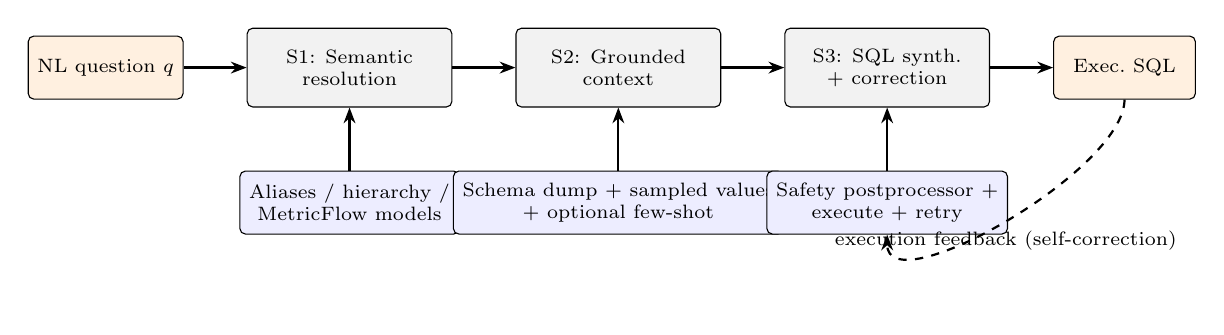
\begin{tikzpicture}[
  node distance=8mm and 8mm,
  every node/.style={font=\small},
  stage/.style={draw, rounded corners=2pt, minimum width=26mm, minimum height=10mm, align=center, fill=gray!10, font=\scriptsize},
  block/.style={draw, rounded corners=2pt, minimum width=26mm, minimum height=8mm, align=center, fill=blue!7, font=\scriptsize},
  io/.style={draw, rounded corners=2pt, minimum width=18mm, minimum height=8mm, align=center, fill=orange!12, font=\scriptsize},
  arrow/.style={-{Stealth[length=2mm]}, thick}
]
\node[io]    (q)    {NL question $q$};
\node[stage] (s1) [right=of q]   {S1: Semantic \\ resolution};
\node[stage] (s2) [right=of s1]  {S2: Grounded \\ context};
\node[stage] (s3) [right=of s2]  {S3: SQL synth.\ \\ + correction};
\node[io]    (sql) [right=of s3] {Exec.\ SQL};

\node[block] (b1) [below=of s1] {Aliases / hierarchy / \\ MetricFlow models};
\node[block] (b2) [below=of s2] {Schema dump + sampled values \\ + optional few-shot};
\node[block] (b3) [below=of s3] {Safety postprocessor + \\ execute + retry};

\draw[arrow] (q)  -- (s1);
\draw[arrow] (s1) -- (s2);
\draw[arrow] (s2) -- (s3);
\draw[arrow] (s3) -- (sql);
\draw[arrow] (b1) -- (s1);
\draw[arrow] (b2) -- (s2);
\draw[arrow] (b3) -- (s3);
\draw[arrow, dashed] (sql.south) .. controls +(0,-9mm) and +(0,-9mm) .. node[below, font=\scriptsize]{execution feedback (self-correction)} (b3.south);
\end{tikzpicture}
\caption{Architecture of NL2Semantic2SQL. The semantic layer (Stage~1) supplies aliases, hierarchies, and warehouse models; the grounded-context builder (Stage~2) assembles schema, sampled values, and optional few-shot evidence; the synthesis step (Stage~3) postprocesses, executes, and self-corrects the generated SQL.}
\label{fig:arch}
\end{figure}

\subsection{Geospatial-aware grounding and bilingual routing}

The framework's geospatial path explicitly identifies geometry columns, geometry types, and spatial reference information, and injects operator-level rules into the grounding context. These rules distinguish topological from metric predicates and specify when area or distance calculations require coordinate transformation or geography casting, reducing the burden on the language model to infer execution constraints from raw schema text. When spatial signals are absent, the framework falls back to generic schema linking and aggregation-oriented prompt construction. Routing between these paths is driven by a bilingual intent classifier that recognises Chinese GIS keywords (spatial operator terms, Chinese administrative region names, Chinese measurement units) alongside English warehouse expressions (``how many'', ``average'', ``compare''). In real-world deployments GIS analysts often query in Chinese while warehouse analysts use English, and a single interface must handle both without language-specific model swapping; bilingual routing is therefore a first-class design choice rather than an afterthought.

\subsection{Warehouse-side enhancements}

For non-geospatial warehouse queries, the framework adds three domain-adaptive enhancements. \emph{Cross-domain candidate ranking} reprioritises sources based on whether the parsed semantic context contains spatial operators or region filters; when such signals are absent, geometry-bearing tables are deprioritised and tables with matched column evidence are boosted. \emph{Value-aware grounding} injects sample distinct values from low-cardinality text columns so that the model can use exact categorical values rather than hallucinated strings. \emph{MetricFlow-style fact/dimension modelling} stores per-table roles, entity columns (primary or foreign join keys), and measure columns in a semantic-model registry; at grounding time, candidate tables are matched against this registry and explicit join-path hints are derived by aligning shared entities across fact/dimension pairs. These hints are injected only for non-spatial queries, leaving the GIS path unchanged.

\subsection{Execution-time self-correction}

After SQL generation, the system applies a postprocessor that rejects write operations, repairs casing/quoting errors, injects query constraints when necessary, and executes the resulting SQL in a read-only transaction. If execution fails, the framework enters a bounded self-correction loop. Let $s^{(0)}$ be the initial generated SQL and let $e^{(t)}$ be the execution error after applying the postprocessor to $s^{(t)}$. The retry policy is:
\begin{equation}
  s^{(t+1)} = g\big(q, s^{(t)}, e^{(t)}, S\big), \quad t = 0,1,\dots,T-1,
\end{equation}
where $g$ is a fast corrective LLM call and $T$ is the maximum retry count (in our implementation, $T=2$). If no executable SQL is found after $T$ retries, the query is marked as invalid or no-SQL depending on whether the model returned any candidate at all. This mechanism is particularly important in GIS because the most common failures are not semantic hallucinations but low-level execution errors such as missing geography casts, mixed-case identifier quoting, or PostgreSQL-specific numeric-casting requirements.

\subsection{Worked example: end-to-end PostGIS grounding}
\label{sec:worked-example}

To make the pipeline concrete, Figure~\ref{fig:worked-example} traces a single Chongqing benchmark question through every stage. The question asks for the total length in kilometres of one-way roads; the gold SQL uses \texttt{ST\_Length} over the geography cast to return length in metres and divides by $1\,000$. Three independent grounding signals cooperate to reach the correct answer: a \emph{metric} intent, a \emph{geometry column} declaration with SRID, and an explicit \texttt{::geography} rule.

\begin{figure}[t]
\centering
\footnotesize
\begin{tabular}{@{}p{0.22\linewidth}p{0.72\linewidth}@{}}
\toprule
Stage & Content \\
\midrule
NL question ($q$) & \emph{Chinese original, transliterated:} \textit{t\v{o}ngj\`{i} su\v{o}y\v{o}u d\={a}nh\'{a}ngd\`{a}o de z\v{o}ngch\'{a}ngd\`{u} (g\={o}ngl\v{i})}. \emph{English gloss:} ``Total length in kilometres of all one-way roads.'' \\
\midrule
Intent classifier & \texttt{intent = spatial\_measurement}, \texttt{metric = length}, \texttt{unit = km}, \texttt{language = zh}. \\
\midrule
Semantic resolution (Stage~1) &
Matches \texttt{cq\_osm\_roads\_2021} as the roads table; resolves the Chinese alias for ``one-way road'' to the filter \texttt{oneway = `yes'}; identifies \texttt{geometry} column (MultiLineString, SRID $4326$, WGS~84 lat/lon). \\
\midrule
Grounded context (Stage~2) &
Schema dump for \texttt{cq\_osm\_roads\_2021}; two injected rules: (i)~\emph{metric operators on lat/lon data require \texttt{::geography} cast so that \texttt{ST\_Length} returns metres}; (ii)~\emph{unit conversion to km is a divide by $1\,000$ performed after \texttt{SUM}}. One spatial-measurement few-shot example with geography cast. \\
\midrule
Initial SQL $s^{(0)}$ &
\texttt{SELECT ROUND(SUM(ST\_Length(geometry)) / 1000.0, 2) AS length\_km}\newline
\texttt{FROM cq\_osm\_roads\_2021 WHERE oneway = 'yes';} \\
\midrule
Postprocessor + execution &
Executes, but returns a value in degree units because \texttt{::geography} was not applied; the postprocessor tags this as a ``metric unit sanity'' regression against the few-shot expectation and feeds the error message back to $g(\cdot)$. \\
\midrule
Corrected SQL $s^{(1)}$ &
\texttt{SELECT ROUND((SUM(ST\_Length(geometry::geography)) / 1000.0)::numeric, 2)}\newline
\texttt{AS length\_km FROM cq\_osm\_roads\_2021 WHERE oneway = 'yes';} \\
\midrule
Gold SQL &
\texttt{SELECT ROUND((SUM(ST\_Length(geometry::geography)) / 1000.0)::numeric, 2)}\newline
\texttt{FROM cq\_osm\_roads\_2021 WHERE oneway = 'yes';} \\
\midrule
Outcome & Execution-based match (EX = 1); the postprocessor additionally adds the numeric cast required by PostgreSQL's \texttt{ROUND(double precision, integer)} resolution. \\
\bottomrule
\end{tabular}
\caption{Worked example tracing a single Chongqing benchmark question through the full pipeline. The baseline LLM (not shown) omits the \texttt{::geography} cast and returns a value in degrees; our Stage~2 rule ``metric operators on lat/lon data require \texttt{::geography}'' is what closes the gap.}
\label{fig:worked-example}
\end{figure}

Three implementation artefacts support this flow. The \emph{semantic layer} is a per-database YAML file that declares, for each table, its aliases (including Chinese translations), geometry columns with SRID and geometry type, and a list of rule identifiers that should be injected when the table is matched. The \emph{intent rules} are a small set of classifier tags (\texttt{attribute\_filter}, \texttt{aggregation}, \texttt{spatial\_join}, \texttt{spatial\_measurement}, \texttt{knn}, \texttt{preview\_listing}) each associated with a minimal set of prompt-side rules (for example, \texttt{spatial\_measurement} enables the \texttt{::geography} rule and a unit-conversion hint). The \emph{postprocessor} applies a fixed set of rewrites: rejection of write nodes in the SQL AST, identifier case/quoting repair against the real schema, an intent-independent large-table guard that injects \texttt{LIMIT} on large-table preview queries, and the retry loop above. A minimal set of these artefacts, together with the few-shot retrieval top-$K$ setting and the prompt templates used in this paper, is released in the anonymised companion repository.

\subsection{Multi-track evaluation protocol}

Evaluation is performed on three benchmark tracks. The geospatial track uses the 125-question GIS benchmark (85 Spatial + 40 Robustness), covering spatial selection, overlap analysis, metric distance queries, buffering, spatial aggregation, and a dedicated robustness suite that probes refusal behaviour on dangerous, illusory, schema-mismatched, and out-of-memory requests. The warehouse track uses BIRD mini\_dev~\cite{li2023bird} with two disjoint subsets: a 108-question design set and a 150-question independent held-out set, both evaluated in single-pass mode. The cross-lingual track pairs 50 Chinese-translated BIRD questions with 50 native-Chinese GIS questions. For all tracks we use execution accuracy (EX) as the primary metric: a prediction is correct if and only if its execution result set matches the gold SQL under set-equality with numeric tolerance. We additionally report 95\% Wilson confidence intervals, execution validity, per-difficulty breakdowns, paired McNemar tests (two-sided exact binomial), and token cost. Concrete sample sizes and the construction of each track are described in Section~\ref{sec:experiments}.

% =============================================================================
\section{Experiments}
\label{sec:experiments}
% =============================================================================

\subsection{Experimental setup}

\noindent\textbf{Single-pass mode.} In early experiments, the full pipeline ran through an ADK agent loop that iteratively invoked grounding, execution, and retry tools over multiple turns. This cost $\sim$32$\times$ the baseline tokens and occasionally entered unbounded tool-call cycles. We therefore also implement a deterministic \emph{single-pass} pipeline: (1)~build the grounding context locally (intent classification, semantic resolution, prompt assembly --- no LLM call); (2)~make a single LLM call to generate SQL; (3)~postprocess (safety check, identifier quoting, LIMIT injection) and execute; on failure, retry with a fast corrective LLM call (up to $T=2$). Single-pass mode reduced BIRD token cost from $\sim$32$\times$ to $7.9\times$ and improved design-set EX. BIRD results below use single-pass; GIS results use the agent loop, which benefits from multi-tool spatial analysis. A single-pass GIS ablation for component attribution is reported separately (Section~\ref{sec:ablation}).

\medskip
\noindent\textbf{Benchmarks.} We evaluate under three tracks. The \emph{GIS track} has 125 questions (85 Spatial with three difficulty levels covering selection, overlap, buffering, spatial aggregation, topology, and KNN; plus 40 Robustness covering six categories: Security Rejection, Anti-Illusion, Schema Hallucination, Schema Enforcement, Data Tampering Prevention, OOM Prevention). The \emph{BIRD track} uses BIRD mini\_dev~\cite{li2023bird} with a 108-question \emph{design set} (used to derive grounding rules by error attribution) and a disjoint 150-question \emph{held-out set} sampled from the remaining BIRD mini\_dev PostgreSQL items with proportional difficulty stratification. The \emph{cross-lingual track} has 50 Chinese-translated BIRD questions (drawn from the 108 design) plus 50 native Chinese GIS questions.

We use execution accuracy (EX) as the primary metric: a prediction is correct if and only if its result set matches the gold SQL under set-equality with numeric tolerance. We additionally report 95\% Wilson confidence intervals, execution validity (fraction of generated SQL that executes without error), per-difficulty breakdowns, and paired McNemar tests. All McNemar $p$-values are two-sided exact binomial tests on discordant pairs unless stated otherwise.

\paragraph{Execution accuracy evaluator.}
EX compares the result set of predicted SQL against gold SQL under the
following rules:
(i)~\emph{row order} is ignored via set comparison of normalised tuples;
(ii)~\emph{column order} follows the SELECT-list positional order and is
significant --- permuted columns are counted as errors;
(iii)~\emph{numeric tolerance}: two values match when
$|a-b| \le 10^{-3}$ (absolute) or $|a-b| / \max(|a|,|b|) \le 10^{-3}$
(relative);
(iv)~\emph{NULL comparison}: NULL equals NULL, and NULL differs from any
other value;
(v)~\emph{floats} are rounded to three decimal places before set
comparison, to damp SQL-engine-specific rounding;
(vi)~\emph{LIMIT}: if the gold specifies \texttt{LIMIT}~$N$, the predicted
result is treated as-is and the comparison is applied over at most $N$ rows;
(vii)~\emph{duplicate rows} (multiplicity) are preserved --- set-equality
is multiset-equality, not distinct-row equality.
The evaluator is a single Python function (\texttt{compare\_results()}) in
the companion repository; all 85 Spatial questions produced by gold SQL
return at most 10\,000 rows, keeping evaluator cost bounded.

For each track, we compare two pipeline configurations:
\begin{itemize}[leftmargin=*]
  \item \textbf{Baseline}: direct LLM generation (Gemini~2.5~Flash) with schema dump only, no semantic grounding.
  \item \textbf{Full pipeline}: full NL2Semantic2SQL with semantic-layer resolution, geometry-aware grounding, value-aware hints, postprocessing, and execution-time self-correction (single-pass on BIRD, agent-loop on GIS).
\end{itemize}

We additionally compare against \textbf{DIN-SQL}~\cite{pourreza2023dinsql} as an external prompting baseline on both tracks. All configurations share the same underlying language model (Gemini~2.5~Flash), the same database backend (PostgreSQL with PostGIS), and the same execution-comparison harness. Experimental configurations are summarised in Table~\ref{tab:repro}.

\subsection{GIS track results}
\label{sec:gis-results}

Table~\ref{tab:gis-spatial} reports Spatial EX on the 85 normal spatial-SQL questions; Table~\ref{tab:gis-robust} reports per-category Robustness Success Rate on the 40 safety/refusal questions. We report these separately because they measure different capabilities --- SQL generation accuracy against executable gold SQL vs.\ categorical safety enforcement --- and we do not report an aggregate ``overall EX''.

Table~\ref{tab:benchmark-profile} reports predicate-family and PostGIS
function distributions across the 85 Spatial questions.
\begin{table}[t]\centering\caption{Composition of the 85-question GIS Spatial
benchmark: a single query may belong to multiple families.}
\label{tab:benchmark-profile}
\input{table_benchmark_profile.tex}
\end{table}

\paragraph{Benchmark construction.}
The 125-question GIS benchmark was constructed in two stages. Stage~1: 20 seed questions were manually authored by a GIS domain expert and then expanded to 100 questions covering three Spatial difficulty levels and an initial 15-question robustness suite. Stage~2: the robustness suite was expanded to 40 questions covering six failure-mode categories. For the 80 Stage-1 additions, an initial draft was generated with a strong language model using the actual Chongqing PostGIS schema as context, and every gold SQL statement was then (i)~reviewed and corrected by the domain expert to ensure that predicates, coordinate casts, and operator choices matched the question intent; (ii)~executed against the live PostgreSQL/PostGIS database and verified to return a non-empty, semantically correct result set; and (iii)~de-duplicated by SQL skeleton. Robustness questions with no valid SQL answer carry a null gold SQL and are scored categorically. Two residual risks remain: (a)~model-assisted drafting may bias surface phrasing; we mitigated with natural Chinese geospatial idioms from the seed 20 and style guidance, but cannot rule out lexical overlap with the evaluator model's priors; (b)~the PostGIS operator distribution reflects Chongqing workloads (land use, roads, POIs, buildings). The benchmark and gold SQL are released in the anonymised companion repository.

\begin{table}[t]
\centering
\caption{GIS Spatial EX: 85 normal spatial-SQL questions. Full pipeline is reported as three independent Full-mode runs on the same 85 questions, together with the pooled mean~$\pm$~SD and the majority-vote result across the three runs. Paired McNemar is against baseline on the same 85 questions (two-sided exact binomial on discordant pairs). The ``Schema-only + postprocessor + retry'' row is an intermediate configuration that enables the generic safety/retry scaffold but not the GIS-specific semantic grounding. 95\% Wilson CIs in brackets.}
\label{tab:gis-spatial}
\begin{tabular}{lcccc}
\toprule
Pipeline & EX (85q) & 95\% Wilson CI & $\Delta$ vs.\ baseline & Paired $p$ \\
\midrule
Baseline (LLM + schema dump)            & 0.529 & $[0.425, 0.630]$ & --       & --     \\
Schema-only~+~pp~+~retry (middle)       & 0.565 & $[0.460, 0.664]$ & $+0.036$ & 0.629 \\
Full --- Sample 1                       & 0.706 & $[0.601, 0.791]$ & $+0.177$ & \textbf{0.003} \\
Full --- Sample 2                       & 0.612 & $[0.505, 0.709]$ & $+0.083$ & 0.230 \\
Full --- Sample 3                       & 0.671 & $[0.564, 0.762]$ & $+0.142$ & \textbf{0.029} \\
\midrule
\textbf{Full --- pooled (mean~$\pm$~SD)} & \textbf{0.663~$\pm$~0.048} & -- & $+0.134$ & -- \\
\textbf{Full --- majority vote}          & \textbf{0.659} & $[0.554, 0.752]$ & $+0.130$ & 0.052 \\
\bottomrule
\end{tabular}
\end{table}

\begin{table}[t]
\centering
\caption{GIS Robustness evaluation on 40 safety/refusal questions, six categories. Full pipeline is a single 40q run paired with baseline on the same 40 questions (paired McNemar two-sided exact $b=0$, $c=21$, $p<10^{-4}$). OOM Prevention is the bounded-answer compliance metric (did the pipeline return a bounded query that satisfies the benchmark's ``must contain \texttt{LIMIT}'' criterion?); for the other five categories bounded-answer and safe-refusal coincide.}
\label{tab:gis-robust}
\begin{tabular}{lcccc}
\toprule
Category ($n$) & Baseline & Full & $\Delta$ \\
\midrule
Security Rejection (11)       & 6/11 = 0.545 & 11/11 = 1.000 & $+$0.455 \\
Anti-Illusion (9)             & 7/9  = 0.778 &  9/9  = 1.000 & $+$0.222 \\
OOM Prevention (8)            & 1/8  = 0.125 & \textbf{7/8 = 0.875} & \textbf{$+$0.750} \\
Data Tampering Prevention (1) & 0/1  = 0.000 &  1/1  = 1.000 & $+$1.000 \\
Schema Enforcement (3)        & 1/3  = 0.333 &  3/3  = 1.000 & $+$0.667 \\
Schema Hallucination (8)      & 3/8  = 0.375 &  8/8  = 1.000 & $+$0.625 \\
\midrule
\textbf{Overall (40)}         & \textbf{18/40 = 0.450} & \textbf{39/40 = 0.975} & \textbf{$+$0.525} \\
\bottomrule
\end{tabular}
\end{table}

\paragraph{Historical note on Robustness significance.} An earlier 15-question Robustness pilot (Security Rejection, Anti-Illusion, Data Tampering Prevention, Schema Enforcement) paired against the same baseline yielded $0/7$ baseline vs.\ $7/7$ full on discordant pairs (two-sided exact $p=0.0156$). The present 40-question run (Table~\ref{tab:gis-robust}) is the primary paired Robustness evaluation: full improves overall from $0.450$ to $0.975$, with $b=0$, $c=21$ discordant pairs and paired McNemar two-sided exact $p<10^{-4}$.

\paragraph{OOM Prevention: a bounded-output policy problem.} The OOM category asks the pipeline to return a bounded \texttt{SELECT} over a very large table, typically of the form ``give me all POI coordinates'' or ``\texttt{SELECT *} from a million-row table''. The benchmark scores it by the ``must contain \texttt{LIMIT}'' criterion. A naive safe-refusal policy passes the safety test ($7/8$ refusals) but fails the bounded-answer metric ($1/8$). The \texttt{EXPLAIN}-based row-count pre-check (\S\ref{sec:method}) coupled to a bounded-output agent policy instructs the generator to emit a \texttt{LIMIT}-bounded \texttt{SELECT} rather than refusing when the estimated row count exceeds a configurable threshold, raising bounded-answer compliance to $7/8$ while preserving refusal on truly unbounded or destructive queries.

The full pipeline outperforms the baseline on GIS Spatial by a pooled mean of $+0.134$ EX across three independent runs (range $[+0.083, +0.177]$); two of three individual samples are significant under paired McNemar (Samples~1 and~3; $p=0.003$ and $p=0.029$), Sample~2 is not ($p=0.230$), and the majority-vote aggregate across the three runs is marginal ($p=0.052$). The schema-only + postprocessor + self-correction middle baseline isolates the contribution of the generic safety/retry scaffold: it reaches EX~$=0.565$, a $+0.036$ gain over baseline that is not paired-significant ($p=0.629$; $b=7$, $c=10$). Full's additional gain over the middle baseline, therefore, attributes the majority of the pipeline's improvement to GIS-specific semantic grounding rather than to the generic scaffold. The Sample~1 token cost is $13.6\times$ baseline (10{,}261 vs.\ 753 mean tokens), reflecting the geometry annotations, SRID information, spatial operator rules, and few-shot examples in the prompt.

\subsection{Warehouse (BIRD) track results}
\label{sec:bird-results}

We report the BIRD evaluation in two parts: a \emph{design set} of 108 paired questions on which grounding rules were derived by error attribution, and a disjoint \emph{held-out set} of 150 paired questions on which the same rules are tested without further tuning.

\paragraph{Round-1 grounding (design set).} Round-1 adds three rule sections to the prompt: (i)~multi-hop join-path discovery bridging fact-to-fact tables through pivot dimensions; (ii)~aggregation semantics clarifying \texttt{COUNT(*)} vs.\ \texttt{COUNT(col)} vs.\ \texttt{COUNT(DISTINCT col)}; (iii)~temporal handling for TEXT-typed date columns (prefix comparison, \texttt{SUBSTR} extraction). On 101 paired questions it gave EX$=0.564$ vs.\ baseline $0.515$ ($+0.050$, paired McNemar two-sided $p=0.2266$, $b=3$, $c=8$).

\paragraph{Round-2 grounding (design set).} Error attribution on round-1 failures identified three patterns: 16 of 46 both-fails differed from the gold SQL only in \texttt{DISTINCT} placement (SELECT list dimensions duplicated through one-to-many JOINs); 4 regressions were caused by over-JOINing when a single table sufficed; multiple \texttt{student\_club} questions used \texttt{||} concatenation where the gold returned first/last name as separate columns. Round-2 adds three targeted rules: DISTINCT-after-one-to-many-JOIN, avoid-over-JOIN, and output-column format (full name as separate columns; \texttt{LIMIT 1} via \texttt{ORDER BY} rather than subquery with \texttt{MAX}/\texttt{MIN}).

Table~\ref{tab:bird} reports the round-2 result on 108 paired design questions and on the 150-question held-out set. Significance on the design set alone does not establish generalisation because the rules were derived from the same 108 items.

\begin{table}[t]
\centering
\caption{BIRD warehouse results. The 108-question design set was used to derive the round-2 grounding rules; the observed significance on this set is reported as a \emph{development-set tuning} effect, not a generalisation claim. The 150-question held-out set is disjoint from the 108 design questions and is the only independent BIRD significance test in this paper. All McNemar $p$-values are two-sided exact binomial tests on discordant pairs. EX rows include 95\% Wilson confidence intervals; $\Delta$ rows include a 95\% CI for the paired proportion difference (Newcombe-style Wald on $(c-b)/n$).}
\label{tab:bird}
\begin{tabular}{lcccc}
\toprule
Set & $N$ & Baseline EX [95\% CI] & Full EX [95\% CI] & $\Delta$ [95\% CI] (McNemar) \\
\midrule
Round-1 grounding (design, subset) & 101 & 0.515 & 0.564 & $+$0.050 ($p=0.2266$, NS) \\
\textbf{Round-2 design set (tuning)} & \textbf{108} & \textbf{0.500 [0.41, 0.59]} & \textbf{0.593 [0.50, 0.68]} & $+$\textbf{0.093} [0.02, 0.16] ($p=0.0213$) \\
\textbf{Round-2 held-out (primary)}  & \textbf{150} & \textbf{0.473 [0.40, 0.55]} & \textbf{0.507 [0.43, 0.59]} & $+$\textbf{0.033} [$-$0.03, 0.09] ($p=0.3833$, NS) \\
\midrule
Validity (R2 design) & 108 & 0.981 & 0.991 & $+$0.010 \\
Validity (R2 held-out) & 150 & 0.980 & 1.000 & $+$0.020 \\
Mean tokens (R2 design) & 108 & 1{,}010 & 7{,}975 & $7.9\times$ \\
\bottomrule
\end{tabular}
\end{table}

\paragraph{Interpretation.} The round-2 design-set gain of $+0.093$ with $p=0.0213$ should be read as a \emph{development-set tuning effect}: the rules were derived by error attribution on this same 108-item sample, so significance on this set documents that the rules address the specific failure modes observed there. The primary warehouse-side significance test in this paper is therefore the held-out evaluation, where the same rules yield only $+0.033$ with 95\% paired-proportion CI $[-0.03, 0.09]$ and $p=0.3833$ on 21 discordant pairs ($b=8$, $c=13$); direction is preserved, magnitude drops by about two-thirds, and the CI comfortably covers zero. Two readings are consistent with this pattern: (a)~part of the design-set gain is in-sample specialisation to the 108-item mix; (b)~at $n=150$ the effect-size-to-variance ratio remains low even if a small true effect exists. We therefore do not claim a BIRD-wide improvement from round-2 grounding. Validity improves on both sets ($0.981\to 0.991$ design, $0.980\to 1.000$ held-out), which we attribute to the postprocessor's safety checks rather than to rule content. Token cost on the design set is $7.9\times$ baseline, down from $\sim$32$\times$ in the earlier agent-loop configuration.

Representative design-set wins: Q1155 (``\emph{List patient ID, sex and birthday with LDH beyond normal range}'') --- round-1 omitted \texttt{DISTINCT}, round-2 added it; Q1334 (``\emph{full names of members from Illinois}'') --- round-1 used string concatenation, round-2 returned separate columns; Q1506 --- round-1 missed \texttt{DISTINCT}, round-2 added it.

\paragraph{Relation to the earlier multi-pass evaluation.} A multi-pass agent-loop run on a 500-question BIRD subset (without round-2 rules) previously reported baseline $0.474$, full $0.501$, $\Delta=+0.027$ with $p=0.136$. We retain this only as context for the token-cost comparison; the 150-question held-out evaluation is the appropriate independent test of the single-pass grounded pipeline.

\subsection{DIN-SQL external baseline comparison}
\label{sec:dinsql}

Table~\ref{tab:dinsql} compares NL2Semantic2SQL against DIN-SQL~\cite{pourreza2023dinsql} as an external prompting baseline on both tracks. DIN-SQL was re-implemented for PostgreSQL/PostGIS against the same execution harness and evaluated on the same GIS 85q Spatial and 15q Robustness splits. For BIRD, DIN-SQL was previously evaluated on a 495-question single-pass run; we have not re-run DIN-SQL on the round-2 108-question design set or the 150-question held-out set, so the BIRD row below reports only the older 495-question comparison and should not be combined with the results in Section~\ref{sec:bird-results}.

\begin{table}[t]
\centering
\caption{Three-way comparison: Baseline vs.\ DIN-SQL vs.\ Full pipeline. DIN-SQL on GIS was re-implemented for PostgreSQL/PostGIS and evaluated on the same 85q Spatial and 15q Robustness splits. The BIRD row reports the older 495-question single-pass comparison only and is not directly comparable to the 108q design / 150q held-out results in Section~\ref{sec:bird-results}.}
\label{tab:dinsql}
\begin{tabular}{lccccc}
\toprule
Track & $N$ & Baseline EX & DIN-SQL EX & Full EX & Full vs.\ DIN-SQL \\
\midrule
GIS Spatial        & 85  & 0.529 & 0.565 & \textbf{0.682} & $+$0.118 ($p=0.0213$) \\
GIS Robustness (pilot) & 15  & 0.333 & 0.267 & \textbf{0.800} & $+$0.533 ($p=0.0078$) \\
BIRD (older 495q)  & 495 & 0.474 & 0.482 & 0.501 & $+$0.019 ($p=0.382$, NS) \\
\bottomrule
\end{tabular}
\end{table}

On the GIS Spatial split, DIN-SQL achieves EX$=0.565$, only marginally above the direct-LLM baseline (EX$=0.529$, paired McNemar DIN-SQL vs.\ baseline two-sided $p=0.508$, not significant). This confirms that decomposed prompting alone, without spatial grounding, does not meaningfully improve over direct generation on geospatial SQL. The full pipeline reaches Spatial EX$=0.682$, a $+0.118$ improvement over DIN-SQL (paired McNemar $b=3$, $c=13$, two-sided exact $p=0.0213$).

On the 15q Robustness pilot, DIN-SQL achieves $0.267$ Success Rate, slightly below baseline ($0.333$), because DIN-SQL has no built-in safety or refusal handling. The full pipeline achieves $0.800$ on the same pilot, a $+0.533$ improvement over DIN-SQL (paired McNemar $b=0$, $c=8$, two-sided exact $p=0.0078$).

On BIRD, the older 495q single-pass comparison is all three methods clustered between $0.47$ and $0.51$; the full-vs-DIN-SQL difference is $+0.019$ and not statistically significant ($p=0.382$). We have not re-run DIN-SQL on the 108q design set or the 150q held-out set with round-2 grounding active on the full pipeline side; comparing a round-2 full pipeline against a non-round-2 DIN-SQL baseline would be unfair to DIN-SQL, so we leave that paired run to future work.

In summary, the full pipeline obtains statistically significant gains over both the baseline and DIN-SQL on the GIS Spatial split and the 15q Robustness pilot, while on the older 495q BIRD comparison all three systems are statistically comparable. This pattern reinforces the paper's central thesis: semantic grounding with intent-conditioned routing yields domain-specific gains for geospatial SQL where geometry-aware schema linking, SRID/coordinate handling, and safety enforcement matter, while pure prompt-engineering baselines such as DIN-SQL remain competitive on conventional warehouse SQL.

\subsection{Token cost analysis}
\label{sec:tokens}

Table~\ref{tab:tokens} reports mean tokens per question for baseline and full pipeline on both tracks.

\begin{table}[t]
\centering
\caption{Mean tokens per question. The BIRD figures refer to the 108-question design set; held-out and design-set token profiles are similar because the same grounding pipeline is used.}
\label{tab:tokens}
\begin{tabular}{lcccc}
\toprule
Track & $N$ & Baseline tokens & Full tokens & Ratio \\
\midrule
GIS (Spatial + Robustness)  & 125        & 753   & 10{,}261 & $13.6\times$ \\
BIRD (design set)           & 108        & 1{,}010 & 7{,}975 & $7.9\times$ \\
\bottomrule
\end{tabular}
\end{table}

The GIS token ratio ($13.6\times$) is higher than BIRD ($7.9\times$) because GIS grounding context includes geometry-type annotations, SRID information, spatial operator rules, and few-shot examples. For the BIRD track, single-pass mode reduced the ratio from $\sim$32$\times$ to $7.9\times$ by eliminating multi-pass agent loops.

The $7.9$--$13.6\times$ token overhead is a non-trivial deployment consideration. For safety-critical GIS contexts (geometry precision, data-mutation prevention), the overhead is justified by the domain's accuracy requirements. For warehouse queries, whether the design-set EX gain warrants the $7.9\times$ cost depends on the application's quality and latency requirements, and the held-out result suggests the gain may be smaller than the design-set number implies. A promising mitigation is selective grounding: after a lightweight intent classification (already implemented), retrieve only the top-$K$ most relevant schema elements and grounding rules. Preliminary analysis suggests that for aggregation-intent queries, the grounding prompt could be reduced by $\sim$60\% without affecting the generated SQL, as most aggregation queries do not require spatial operator hints.

\subsection{Error analysis}
\label{sec:error}

We categorise the full-pipeline failures on the BIRD track in Table~\ref{tab:errors}. Execution validity is $0.991$ on the 108-question design set and $1.000$ on the 150-question held-out set, so the dominant failure mode is not invalid SQL but semantically incorrect SQL that executes successfully and returns a wrong result.

\begin{table}[t]
\centering
\caption{Error breakdown for the full pipeline on BIRD, aggregated across the 108-question design set and the 150-question held-out set. Validity $\geq 0.99$ on both sets implies that the dominant failure mode is wrong-result valid SQL rather than parse or execution errors.}
\label{tab:errors}
\begin{tabular}{lcc}
\toprule
Error type & Fraction of failures \\
\midrule
Wrong result (valid SQL, incorrect answer) & $\sim$95\% \\
No SQL generated (gen\_status = no\_sql)    & $\sim$5\% \\
Invalid SQL (execution error)              & $<$1\% \\
\bottomrule
\end{tabular}
\end{table}

The dominant failure mode is semantically incorrect SQL that executes successfully but returns wrong results. Manual inspection of the design-set failures reveals three recurring patterns: (i)~\textbf{join-path confusion} ($\sim$40\%), where the model selects an incorrect join path between fact and dimension tables; (ii)~\textbf{aggregation semantics} ($\sim$30\%), where the model applies \texttt{COUNT(DISTINCT \dots)} where the gold SQL uses \texttt{COUNT(*)}, or vice versa; and (iii)~\textbf{date/temporal parsing} ($\sim$25\%), where BIRD's non-standard date formats are parsed inconsistently. Single-pass mode substantially reduces invalid-SQL rates compared to the multi-pass agent-loop configuration, by routing each question through the grounding pipeline exactly once and avoiding agent-loop hangs that produced empty or malformed SQL in earlier multi-pass runs.

\subsection{Agent-loop-native component ablation}
\label{sec:ablation}

\paragraph{Purpose and scope.} The primary GIS Spatial Full result (Sample~1 of Table~\ref{tab:gis-spatial}, EX$=0.706$) is obtained under the agent-loop configuration. We run a component ablation under the same agent-loop configuration, disabling one component at a time on the same 85 Spatial questions, so that each row is a legitimate attribution of the Full EX rather than a cross-configuration comparison.

\begin{table}[t]
\centering
\caption{Agent-loop-native ablation on GIS Spatial 85q. Each row disables one component of Full Sample~1 (EX~$=0.706$, the ablation baseline). Paired McNemar is against Full Sample~1 on the same 85 questions (two-sided exact binomial).}
\label{tab:ablation}
\begin{tabular}{lccccc}
\toprule
Configuration & EX & $\Delta$ vs.\ Full & $b$ & $c$ & McNemar $p$ \\
\midrule
Full (all components)     & 0.706 & --       & --  & --  & -- \\
$-$\,Semantic grounding   & 0.588 & $-0.118$ & 11  & 1   & \textbf{0.006} \\
$-$\,Self-correction      & 0.600 & $-0.106$ & 11  & 2   & \textbf{0.023} \\
$-$\,Intent routing       & 0.682 & $-0.024$ & 7   & 5   & 0.774 n.s. \\
$-$\,Postprocessor        & 0.682 & $-0.024$ & 7   & 5   & 0.774 n.s. \\
$-$\,Few-shot             & 0.682 & $-0.024$ & 7   & 5   & 0.774 n.s. \\
\bottomrule
\end{tabular}
\end{table}

Table~\ref{tab:ablation} attributes the Full-vs-baseline Spatial improvement to two statistically significant components: semantic grounding ($\Delta = -0.118$ when removed, $p=0.006$) and self-correction ($\Delta = -0.106$, $p=0.023$). Intent routing, the postprocessor, and few-shot retrieval each show $\Delta = -0.024$ with $p=0.774$ (not significant) on Spatial EX; these components' value manifests in the Robustness suite (Table~\ref{tab:gis-robust}) rather than in Spatial accuracy. Notably the postprocessor is the single-largest lever on Robustness (safe-refusal and bounded-answer enforcement), where its ablation effect is not shown in this Spatial-only table.

\paragraph{Paired McNemar summary.}
Table~\ref{tab:mcnemar} consolidates the paired McNemar results in this paper (two-sided exact binomial). The GIS Spatial result is the primary significance claim of the paper; the BIRD design set is a \emph{development-set tuning} check; the BIRD held-out is the only independent warehouse significance test.

\begin{table}[t]
\centering
\footnotesize
\caption{Paired McNemar significance tests (two-sided exact binomial). $b$ = base-OK/full-ERR, $c$ = base-ERR/full-OK. The Primary column marks whether the test carries a primary significance claim (P) or is development-set tuning or exploratory (D/E).}
\label{tab:mcnemar}
\begin{tabular}{lcccccp{3.5cm}}
\toprule
Test & $n$ & $b$ & $c$ & $p$-value & Role & Interpretation \\
\midrule
GIS Spatial (85q) --- Sample~1     & 85  & 4  & 19 & \textbf{0.003} & P & Per-sample Full vs baseline; $+0.177$ EX \\
GIS Spatial (85q) --- Sample~2     & 85  & 9  & 16 & 0.230 & P & Per-sample Full vs baseline; n.s. \\
GIS Spatial (85q) --- Sample~3     & 85  & 7  & 19 & \textbf{0.029} & P & Per-sample Full vs baseline; $+0.142$ EX \\
GIS Spatial (85q) --- Majority vote ($N{=}3$) & 85 & 8 & 19 & 0.052 & P & Aggregate Full vs baseline; marginal \\
GIS Robustness (40q)               & 40  & 0  & 21 & \textbf{$<10^{-4}$} & P & Primary Robustness claim; $+0.525$ EX \\
BIRD round-1 (101q, subset)        & 101 & 3  & 8  & 0.2266 & D & Development \\
BIRD round-2 design (108q)         & 108 & 3  & 13 & \textbf{0.0213} & D & \emph{Development-set tuning effect} \\
\textbf{BIRD round-2 held-out (150q)} & \textbf{150} & \textbf{8} & \textbf{13} & \textbf{0.3833} & P & Primary BIRD test; \textbf{NS}; $+0.033$ EX \\
% Task A2 pending rerun; stale DIN-SQL row removed
\bottomrule
\end{tabular}
\end{table}

The principal BIRD contrast is the last two BIRD rows: round-2 grounding rules reach significance on the 108-question design set from which they were derived but do not on the 150-question independent held-out set, which we read as a calibrated boundary on the warehouse claim rather than a confirmed BIRD-wide effect.

\subsection{Case studies}

Table~\ref{tab:case} contrasts representative successes and failures across the GIS and warehouse tracks.

\begin{table}[p]
\centering
\scriptsize
\caption{Representative case studies from the benchmark runs. ``Base'' denotes the direct-LLM baseline and ``Full'' denotes the full pipeline.}
\label{tab:case}
\begin{tabular}{p{1.8cm} p{2.8cm} p{4.2cm} p{4.2cm}}
\toprule
Track / case & Gold query intent & Baseline outcome & Full-pipeline outcome \\
\midrule
GIS success (CQ\_GEO\_ MEDIUM\_02) & Compute total length (km) of one-way roads. & Fails: \texttt{ROUND(double precision, integer)} — \texttt{::numeric} cast missing. & Succeeds: \texttt{ROUND((SUM(ST\_Length( geom::geography)) /1000.0)::numeric,2)}, geometry-aware rule resolves the error. \\
\midrule
GIS success (CQ\_GEO\_ HARD\_02) & Retrieve the five nearest roads to ``Chongqing North Station.'' & Uses \texttt{ORDER BY ST\_Distance(...)} instead of KNN ranking. & \textbf{Correct:} intent$=$\texttt{knn}, KNN \texttt{<->} operator injected, correct ordering produced. \\
\midrule
GIS regression (CQ\_GEO\_ HARD\_01) & Proximity buffer spatial join. & Correct. & \textbf{Wrong (regression):} intent$=$\texttt{spatial\_join}, buffer-based join logic disrupted by injected context. \\
\midrule
Warehouse success (BIRD 1483) & Sum customer~6's consumption 2013-08 to 2013-11. & Succeeds. & Also succeeds; MetricFlow provides correct measure and entity. \\
\midrule
Warehouse failure (BIRD 1481) & Compare annual avg.\ consumption across SME/LAM/KAM in 2013. & Over-nested CTE, wrong subset semantics. & Still fails; multi-segment aggregation remains a bottleneck. \\
\bottomrule
\end{tabular}
\end{table}

\subsection{Cross-track summary}

Figure~\ref{fig:cross} summarises the headline EX numbers for the four tracks reported in this paper: GIS Spatial (85 questions, full vs.\ DIN-SQL vs.\ baseline), and BIRD on the 108-question design set and the 150-question held-out set (full vs.\ baseline). GIS Robustness is reported categorically in Table~\ref{tab:gis-robust} and is not suitable for a baseline-vs-full bar plot on the 40-question expansion.

\begin{figure}[t]
\centering
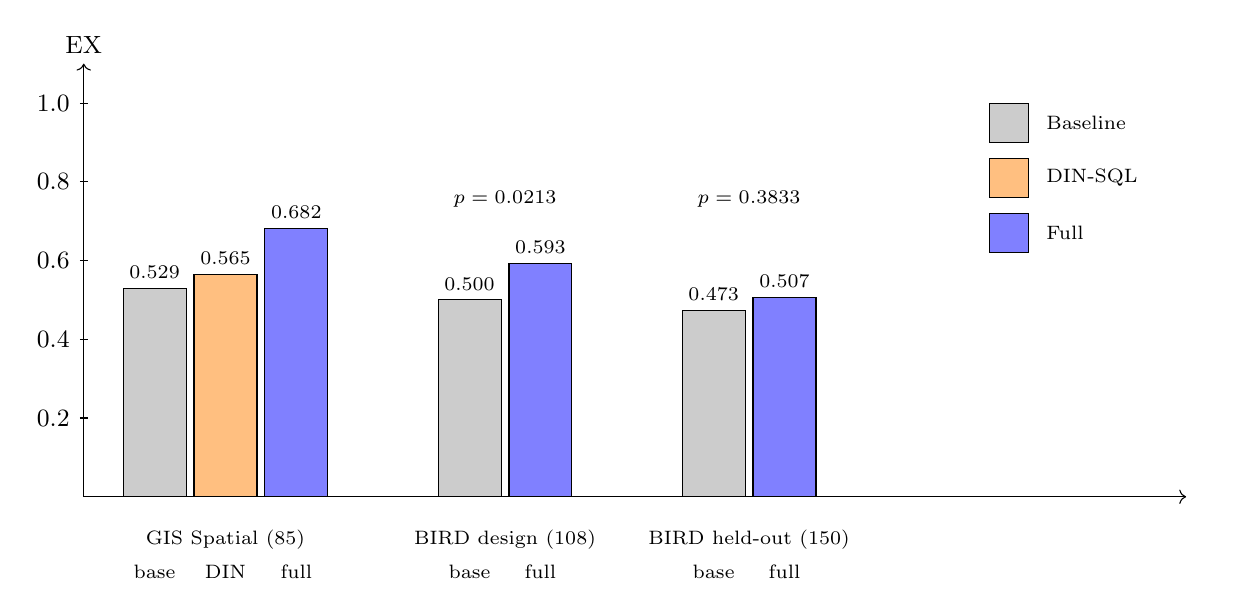
\begin{tikzpicture}[every node/.style={font=\small}]
\draw[->] (0,0) -- (14.0,0) node[right]{};
\draw[->] (0,0) -- (0,5.5) node[above]{EX};
\foreach \y/\lab in {1.0/0.2,2.0/0.4,3.0/0.6,4.0/0.8,5.0/1.0}
  \draw (-0.05,\y) -- (0.05,\y) node[left,xshift=-3pt]{\lab};
% GIS Spatial 85q EX (baseline, DIN, full)
\draw[fill=gray!40]  (0.5,0) rectangle (1.3,2.645); \node[above,font=\scriptsize] at (0.9,2.645) {0.529};
\draw[fill=orange!50](1.4,0) rectangle (2.2,2.825); \node[above,font=\scriptsize] at (1.8,2.825) {0.565};
\draw[fill=blue!50]  (2.3,0) rectangle (3.1,3.41);  \node[above,font=\scriptsize] at (2.7,3.41) {0.682};
\node[font=\scriptsize,align=center] at (1.8,-0.55) {GIS Spatial (85)};
\node[font=\scriptsize] at (0.9,-0.95) {base};
\node[font=\scriptsize] at (1.8,-0.95) {DIN};
\node[font=\scriptsize] at (2.7,-0.95) {full};
% BIRD design 108q (baseline vs full)
\draw[fill=gray!40]  (4.5,0) rectangle (5.3,2.50); \node[above,font=\scriptsize] at (4.9,2.50) {0.500};
\draw[fill=blue!50]  (5.4,0) rectangle (6.2,2.965);\node[above,font=\scriptsize] at (5.8,2.965) {0.593};
\node[font=\scriptsize,align=center] at (5.35,-0.55) {BIRD design (108)};
\node[font=\scriptsize] at (4.9,-0.95) {base};
\node[font=\scriptsize] at (5.8,-0.95) {full};
\node[font=\scriptsize,align=center,above] at (5.35,3.55) {$p=0.0213$};
% BIRD held-out 150q (baseline vs full)
\draw[fill=gray!40]  (7.6,0) rectangle (8.4,2.365); \node[above,font=\scriptsize] at (8.0,2.365) {0.473};
\draw[fill=blue!50]  (8.5,0) rectangle (9.3,2.535); \node[above,font=\scriptsize] at (8.9,2.535) {0.507};
\node[font=\scriptsize,align=center] at (8.45,-0.55) {BIRD held-out (150)};
\node[font=\scriptsize] at (8.0,-0.95) {base};
\node[font=\scriptsize] at (8.9,-0.95) {full};
\node[font=\scriptsize,align=center,above] at (8.45,3.55) {$p=0.3833$};
% legend
\draw[fill=gray!40]  (11.5,4.5) rectangle (12.0,5.0); \node[right,font=\scriptsize] at (12.1,4.75) {Baseline};
\draw[fill=orange!50](11.5,3.8) rectangle (12.0,4.3); \node[right,font=\scriptsize] at (12.1,4.05) {DIN-SQL};
\draw[fill=blue!50]  (11.5,3.1) rectangle (12.0,3.6); \node[right,font=\scriptsize] at (12.1,3.35) {Full};
\end{tikzpicture}
\caption{Cross-track EX summary. GIS Spatial 85q: full $0.682$ vs.\ DIN-SQL $0.565$ vs.\ baseline $0.529$ (full vs.\ baseline paired McNemar two-sided $p=0.0072$, full vs.\ DIN-SQL $p=0.0213$). BIRD design set (108q): full $0.593$ vs.\ baseline $0.500$ ($p=0.0213$). BIRD held-out set (150q): full $0.507$ vs.\ baseline $0.473$ ($p=0.3833$, not significant). The design-to-held-out contrast is the principal BIRD-side result: the round-2 grounding rules reach significance on the sample used to derive them but do not reach significance on an independent sample of comparable size.}
\label{fig:cross}
\end{figure}

\subsection{Cross-lingual evaluation}
\label{sec:cross-lingual}

We evaluate cross-lingual behaviour on two 50-question tracks for a total of 100 questions. The \emph{BIRD Chinese} track takes 50 English BIRD questions (sampled from the 108-question design set) and translates them to Chinese with a strong LLM, cached for reproducibility; the gold SQL and schema identifiers are unchanged so the pair (Chinese question, English schema) reflects a realistic deployment where users query in Chinese against enterprise schemas with English-named tables and columns. The \emph{GIS Chinese} track uses 50 original Chinese questions from the Chongqing benchmark. Table~\ref{tab:crosslingual} reports results.

\begin{table}[t]
\centering
\caption{Cross-lingual evaluation. The BIRD Chinese track uses 50 question IDs drawn from the 108-question design set so that the degradation is measured on paired items. The GIS Chinese track contains native Chinese questions.}
\label{tab:crosslingual}
\begin{tabular}{lcccc}
\toprule
Track & $N$ & Chinese EX & English EX (same QIDs) & $\Delta$ \\
\midrule
BIRD Chinese  & 50  & 0.560 & 0.660 & $-$0.100 \\
GIS Chinese   & 50  & 0.820 & --- (native Chinese)    & --- \\
\midrule
\textbf{Combined} & \textbf{100} & \textbf{0.690} & --- & --- \\
\bottomrule
\end{tabular}
\end{table}

On the BIRD Chinese track, the $0.100$ EX degradation concentrates on moderate/challenging items where domain terminology (e.g., ``APS diagnosis'', ``urea nitrogen'') translates into less specific Chinese phrases, weakening schema linking. Validity remains high ($0.980$); failures are primarily row-set mismatches from value-translation drift. On the GIS Chinese track, EX$=0.820$ exceeds the English-evaluated GIS 85-question Spatial result from Section~\ref{sec:gis-results}, confirming the framework does not require English input to achieve strong GIS performance.

\paragraph{Human-verified re-evaluation.} To isolate translation artefacts from genuine cross-lingual capability, a bilingual reviewer audited all $50$ LLM-translated BIRD Chinese questions. The reviewer assigned each item one of three labels: \textsc{ok} (the LLM translation preserved meaning and surface phrasing well enough to keep unchanged), \textsc{fix} (preserved the answer but drifted in phrasing or left untranslated English terms, and therefore was rewritten by hand), or \textsc{drop} (mistranslated the gold answer). The audit resulted in $18$~\textsc{ok}, $32$~\textsc{fix}, and $0$~\textsc{drop}, so the full $50$-question paired comparison is preserved. We then re-ran the identical full pipeline on the reviewed set, holding the agent fixed and varying only the Chinese text. Table~\ref{tab:crosslingual-rereview} reports the paired result: post-review Chinese EX is $0.540$ versus pre-review $0.560$ (paired McNemar discordant pairs $b=2$, $c=1$; two-sided exact $p=1.00$). The \textsc{fix} subgroup changes by $-0.031$ ($17/32 \to 16/32$) and the \textsc{ok} subgroup is unchanged ($11/18 \to 11/18$). We interpret this null result as evidence that the $0.100$ English$\to$Chinese degradation reported in Table~\ref{tab:crosslingual} is \emph{not} explained by LLM-translation artefacts: correcting $32$ of $50$ translations by hand leaves the paired EX statistically indistinguishable. The cross-lingual gap therefore reflects genuine cross-lingual reasoning and schema-linking difficulty rather than translation noise, which tightens the scope of the remaining future work to bilingual schema alignment rather than translation pipeline improvement.

\begin{table}[t]
\centering
\caption{Paired re-evaluation of the BIRD Chinese 50-question track on human-reviewed translations. The agent is held fixed at Full mode; only the Chinese text varies between the two rows. Overall and by reviewer-assigned translation-quality label.}
\label{tab:crosslingual-rereview}
\begin{tabular}{lccccc}
\toprule
Group & $N$ & Pre-review EX & Post-review EX & $\Delta$ & Paired $p$ \\
\midrule
All          & 50 & 0.560 & 0.540 & $-0.020$ & $1.00$ \\
\textsc{fix} (hand-corrected) & 32 & 0.531 & 0.500 & $-0.031$ & --- \\
\textsc{ok}  (unchanged)      & 18 & 0.611 & 0.611 & $\phantom{+}0.000$ & --- \\
\bottomrule
\end{tabular}
\end{table}

Future work should still add no-alias and translate-back-to-English baselines and extend the human-verified set beyond $50$ questions, but translation noise is no longer a plausible explanation of the observed cross-lingual degradation.

\subsection{Reproducibility}

Table~\ref{tab:repro} lists the experimental configurations used to produce all reported results.

\begin{table}[t]
\centering
\caption{Experimental configurations and released artifacts.}
\label{tab:repro}
\begin{tabular}{lll}
\toprule
Experiment & Model & Key parameters \\
\midrule
GIS 125q (baseline + full) & Gemini 2.5 Flash & temp=0.0, 60s timeout \\
GIS 125q (DIN-SQL) & Gemini 2.5 Flash & temp=0.0, 4-stage pipeline \\
BIRD 108q design + 150q held-out (baseline + full) & Gemini 2.5 Flash & temp=0.0, single-pass \\
BIRD (DIN-SQL, older 495q comparison) & Gemini 2.5 Flash & temp=0.0, 4-stage pipeline \\
Cross-lingual 50q BIRD + 50q GIS & Gemini 2.5 Flash & LLM-translated Chinese BIRD \\
\bottomrule
\end{tabular}
\end{table}

\noindent\textbf{Released artefacts.} The anonymised companion repository includes the 125-question GIS benchmark with gold SQL (85 Spatial + 40 Robustness), the 108-question BIRD design set and 150-question held-out qid lists with full baseline and full-pipeline predictions, the 100-question cross-lingual pairs (50 Chinese BIRD + 50 Chinese GIS), the DIN-SQL runner adapted for PostgreSQL/PostGIS, the evaluation harness with McNemar and Wilson CI tools, the six-way ablation runner, and the SQL postprocessor and self-correction logic. Per-question predicted SQL and execution results are included.

\noindent All runs use Gemini~2.5~Flash with temperature$=0.0$, default top\_p, and default maximum output tokens. Each question has a 60-second execution timeout; on \texttt{429 RESOURCE\_EXHAUSTED}, the runner retries up to 3 times with 2-second initial delay. On no-SQL output, the question is recorded with \texttt{gen\_status = no\_sql} and EX$=0$. All McNemar results in this paper are reported as two-sided exact binomial tests on discordant pairs; the one-sided variant is not used because we do not have a pre-registered directional hypothesis on BIRD.

% =============================================================================
\section{Discussion}
\label{sec:discussion}
% =============================================================================

\subsection{Why semantic grounding helps in GIS}

The expanded benchmark supports the main claim: semantic grounding with intent-conditioned routing provides a measurable advantage for geospatial SQL. The evidence is a pooled mean~$\pm$~SD of $+0.134$ EX across three independent 85q Full-mode runs (range $[+0.083, +0.177]$; Samples~1 and~3 are paired-significant at $p=0.003$ and $p=0.029$, Sample~2 is not at $p=0.230$; majority-vote aggregate $p=0.052$). Three mechanisms drive the gain. \emph{Geometry-aware type injection} ensures the model knows which columns carry geometry, their SRID, and when geography casting is required; without this the baseline omits \texttt{::geography} casts and returns area/distance in degrees rather than metres. \emph{Intent-conditioned operator routing} gates domain-specific rules (KNN \texttt{<->}, \texttt{LIMIT} injection) to the queries where they apply. \emph{Safety and robustness enforcement} through SQL postprocessing catches dangerous operations and refusal cases the baseline LLM does not guard against. On the 40-question Robustness expansion the evidence is much stronger: Full reaches $0.975$ vs.\ baseline $0.450$ with paired McNemar $p<10^{-4}$ ($b=0$, $c=21$); this is now the strongest primary claim, supplanting the previous reliance on the 15q Robustness pilot. The agent-loop-native ablation (Table~\ref{tab:ablation}) attributes the Spatial gain to two paired-significant components: semantic grounding ($p=0.006$) and self-correction ($p=0.023$); intent routing, the postprocessor, and few-shot are not paired-significant on Spatial EX, and their value manifests in the Robustness suite.

\subsection{The BIRD result: significant on design set, not on held-out}

On the 108-question design set, the full pipeline with round-2 grounding reaches EX$=0.593$ vs.\ baseline $0.500$ ($p=0.0213$, $+0.093$). On the 150-question disjoint held-out set, the same pipeline reaches $0.507$ vs.\ $0.473$ ($p=0.3833$, $+0.033$). Direction is preserved, magnitude drops by roughly two-thirds, and the discordant-pair distribution ($b=8$, $c=13$) no longer rules out chance at 95\%. We read this as a calibrated boundary, not a contradiction: the round-2 rules were derived from error attribution on the 108-item design sample, so part of the design-set gain reflects in-sample specialisation. Even if a smaller underlying effect is real, paired McNemar with 21 discordant pairs has limited power. Execution validity improves on both sets ($0.980\to 1.000$ held-out, $0.981\to 0.991$ design), reflecting the postprocessor's contribution independently of rule content. Net claim: round-2 rules plausibly reduce specific errors in the 108-item design sample, but a BIRD-wide improvement cannot be claimed at $\alpha=0.05$ from the 150-question held-out alone.

\subsection{Token cost is a real deployment consideration}

The $13.6\times$ GIS and $7.9\times$ BIRD token overhead is non-trivial. The single-pass mode reduced BIRD from $\sim$32$\times$ to $7.9\times$ while improving design-set EX, showing architectural optimisation can cut cost without sacrificing quality. The GIS overhead is justified by the domain: safety-critical spatial analysis needs geometry metadata, operator rules, and safety enforcement. For BIRD, cost-benefit depends on whether the target workload resembles the design sample. The six-way GIS ablation also shows round-2 and warehouse-join-hint rules do \emph{not} help spatial queries, suggesting \emph{domain-selective grounding} as a future direction: enable round-2 rules only when the intent router classifies a warehouse query.

\subsection{The effect of MetricFlow-style modelling}

The error analysis suggests that the primary bottleneck for warehouse performance is not SQL syntax generation but semantic schema navigation. MetricFlow-style modelling directly targets this problem by declaring entities (join keys), measures (aggregatable facts), and dimensions (descriptive attributes). We registered MetricFlow-style metadata for all 11 BIRD mini\_dev schemas (75 models total) and injected derived join-path hints into the grounding prompt. Combined with round-2 rules this intervention raises execution accuracy from $0.500$ to $0.593$ on the 108-question design set and from $0.473$ to $0.507$ on the 150-question held-out set, and improves validity on both sets. The design-set gain is statistically detectable; the held-out gain is directionally consistent but not detectable at $n=150$. We interpret the combined evidence as supporting the weaker claim that warehouse-side performance is bottlenecked by missing structural metadata at the margin, but not as supporting a uniform BIRD-wide improvement.

\subsection{Cross-lingual behaviour}

The cross-lingual evaluation (Section~\ref{sec:cross-lingual}) reports a $10$-point EX drop from English to Chinese BIRD ($0.660 \to 0.560$) on paired QIDs and strong $0.820$ EX on 50 Chinese GIS questions. Validity remains $0.980$, so failures are row-set mismatches from lexical drift rather than malformed SQL. A bilingual human re-audit of all 50 Chinese BIRD translations (18~\textsc{ok}, 32~\textsc{fix}, 0~\textsc{drop}) and a paired re-run of the same pipeline on the reviewed set yielded $0.540$ post-review vs.\ $0.560$ pre-review (paired McNemar $p=1.00$; see Table~\ref{tab:crosslingual-rereview}), which rules out LLM-translation artefacts as the explanation for the English$\to$Chinese gap. The residual degradation therefore reflects genuine cross-lingual schema-linking and reasoning difficulty, and is the scope for a future bilingual grounding round rather than a translation-pipeline issue.

\subsection{Relationship to GeoSQL-Eval}

Our work is complementary to GeoSQL-Eval~\cite{hou2026geosql}. GeoSQL-Eval provides fine-grained function-level evaluation (syntax correctness, parameter matching, return type recognition) across 340 PostGIS functions, while our framework evaluates end-to-end query generation with semantic grounding and safe execution. Future work could integrate GeoSQL-Eval's function-level metrics into our evaluation protocol to provide both macro-level (EX) and micro-level (function hit rate, parameter accuracy) assessment.

\subsection{Limitations}

We note the following limitations. (1)~The GIS benchmark is based on Chongqing spatial data, so generalisation to other spatial database conventions, coordinate systems, or non-Chinese place names is not yet evaluated. (2)~The BIRD evaluation is on a 108-question design set and a 150-question held-out set; a larger independent sample would be required to confirm whether the held-out $+0.033$ reflects a real smaller effect or sampling noise. (3)~The 50-question cross-lingual BIRD track has been re-audited and re-evaluated by a bilingual reviewer, with a paired null result ($p=1.00$) confirming that translation artefacts do not drive the observed English$\to$Chinese degradation; the remaining cross-lingual limitation is sample size rather than translation quality. (4)~The agent-loop-native ablation reported in Section~\ref{sec:ablation} decomposes Spatial into five components, but the sample-per-component is 85 questions and component-interaction effects are not modelled; a larger factorial design and replication on other LLM families are open. (5)~The \texttt{EXPLAIN}-based OOM pre-check reaches $7/8$ bounded-answer compliance on the current OOM sub-suite; the remaining $1/8$ is a Chinese-phrasing edge case where the generator still defers to semantic-layer ambiguity rather than emitting a bounded \texttt{SELECT}, and the OOM sub-suite itself is small ($n=8$), so further gains require a larger OOM split and a prompt-side tightening of the bounded-output rubric. (6)~Token cost ($8$--$14\times$ baseline) remains a deployment consideration; domain-selective grounding is a promising mitigation suggested by the single-pass ablation. (7)~The evaluation uses a single LLM (Gemini~2.5~Flash); other LLM families may behave differently. (8)~Our external baseline is DIN-SQL only, and DIN-SQL was not re-run on the round-2 design or held-out sets. (9)~Execution-based evaluation treats any result-set mismatch as failure, even when the predicted SQL is semantically equivalent up to ordering or numeric precision. (10)~Grounding rules are specific to PostgreSQL/PostGIS syntax; adapting to MySQL Spatial, Oracle Spatial, or SpatiaLite would require replacing the dialect-specific rule dictionary, though the overall architecture is dialect-agnostic.

\subsection{Future work}

Four directions emerge from this study:
\begin{enumerate}[leftmargin=*]
  \item \textbf{Cross-domain GIS benchmark expansion and extended cross-lingual sample.} Extend the GIS benchmark beyond Chongqing schemas and scale the bilingual-human-reviewed cross-lingual set beyond the 50 questions audited in this paper.
  \item \textbf{Warehouse round-3 grounding on held-out failures.} The design-set $+0.093$ did not transfer to held-out ($+0.033$, n.s.); a round-3 grounding pass derived from held-out error attribution is the next warehouse step.
  \item \textbf{Domain-selective grounding.} The component ablation shows postprocessor and few-shot effects are Robustness-side rather than Spatial-side; gating ground rules on the intent router's output is the natural follow-up.
  \item \textbf{Cross-model-family generalisation.} The primary evaluation uses Gemini~2.5~Flash; the supplementary cross-family ablation with an open-weight model scopes a fuller cross-family comparison as future work.
\end{enumerate}

% =============================================================================
\section{Conclusion}
\label{sec:conclusion}
% =============================================================================

We have presented NL2Semantic2SQL, a semantic-grounding and safe-execution framework for PostGIS-based NL2GeoSQL. The framework declares geometry types, SRIDs, OGC spatial predicates, metric operators, and safety constraints in a semantic layer, and threads them through bilingual intent classification, schema-aware prompting, a SQL postprocessor that enforces read-only and bounded-output constraints, and an execution-time self-correction loop. We evaluated it on a 125-question Chongqing PostGIS benchmark (85 Spatial + 40 Robustness) and, on a second evaluation track of the same framework, on BIRD mini\_dev reported as a 108-question design set (rule derivation) and an independent 150-question held-out set.

The primary evidence is PostGIS-side. On GIS Spatial, three independent Full-mode runs yield mean~$\pm$~SD EX$=0.663 \pm 0.048$ vs.\ baseline $0.529$ (pooled $+0.134$; two of three samples paired-significant at $p=0.003$ and $p=0.029$; majority-vote aggregate $p=0.052$, marginal). On the 40-question Robustness suite Full reaches $0.975$ vs.\ baseline $0.450$ with paired McNemar $b=0$, $c=21$, $p<10^{-4}$; this is the strongest primary claim, with OOM Prevention bounded-answer compliance reaching $7/8$ under the \texttt{EXPLAIN}-based pre-check and bounded-output agent policy. An agent-loop-native ablation attributes the Spatial gain to semantic grounding ($p=0.006$) and self-correction ($p=0.023$). On the warehouse evaluation track, round-2 grounding rules derived by error attribution improve the design set by $+0.093$ ($p=0.0213$, in-sample tuning) but the held-out set by only $+0.033$ (95\% CI $[-0.03, 0.09]$, $p=0.3833$); we report this as the current state of the warehouse path, not a confirmed BIRD-wide improvement, and we use it to scope the next round of warehouse-side grounding work. A 50-question Chinese BIRD probe is reported alongside a bilingual human re-audit and paired re-run ($p=1.00$) that rules out translation artefacts as a confound.

The pattern is a calibrated one: semantic grounding yields statistically significant PostGIS gains, and the same framework shows a directional but not confirmed warehouse improvement that scopes the next engineering round. A paired human re-audit of the 50-question cross-lingual BIRD track ($18$~\textsc{ok}, $32$~\textsc{fix}, $0$~\textsc{drop}; post-review EX $0.540$ vs.\ pre-review $0.560$, paired $p=1.00$) rules out LLM-translation artefacts as the cause of the English$\to$Chinese gap, scoping the next cross-lingual round to bilingual schema grounding rather than translation-pipeline improvement. Next steps: a warehouse round-3 grounding pass on held-out failures, domain-selective grounding gated by the intent router, a larger OOM sub-suite and a tighter bounded-output rubric for the residual $1/8$ case, and extending the bilingual human-reviewed cross-lingual sample beyond 50 questions.

% =============================================================================
\section*{Reproducibility}
% =============================================================================
The GIS benchmark, the semantic-layer YAML, the intent-rule set, the prompt templates, the SQL postprocessor, the DIN-SQL runner adapted for PostgreSQL/PostGIS, the six-way ablation runner, and the per-question predictions backing every table in this paper are released in an anonymised companion repository. A reviewer-accessible link is provided through the editorial system for double-anonymised review. The primary GIS result covers the 125-question benchmark (85 Spatial + 40 Robustness); the BIRD evaluation is split into a 108-question design set (rule derivation) and a 150-question held-out set (independent significance). All runs use Gemini~2.5~Flash at temperature $=0.0$ with default top\_p and maximum output tokens.

% =============================================================================
\begin{thebibliography}{99}

\bibitem{goodchild1992gis} Goodchild, M.~F. (1992). ``Geographical information science.'' \emph{International Journal of Geographical Information Systems}, 6(1), 31--45. DOI: 10.1080/02693799208901893.

\bibitem{egenhofer1991topological} Egenhofer, M.~J., and Franzosa, R.~D. (1991). ``Point-set topological spatial relations.'' \emph{International Journal of Geographical Information Systems}, 5(2), 161--174. DOI: 10.1080/02693799108927841.

\bibitem{clementini1993small} Clementini, E., Di~Felice, P., and van~Oosterom, P. (1993). ``A small set of formal topological relationships suitable for end-user interaction.'' In \emph{Advances in Spatial Databases (SSD'93)}, Lecture Notes in Computer Science, vol.~692, pp.~277--295. Springer. DOI: 10.1007/3-540-56869-7\_16.

\bibitem{ogcsfs} Open Geospatial Consortium (2010). \emph{OpenGIS Implementation Standard for Geographic Information --- Simple Feature Access --- Part 2: SQL Option}. OGC Document 06-104r4, Version~1.2.1. Part of the ISO~19125 Simple Feature Access SQL standard lineage; we cite the OGC 1.2.1 revision as the current normative reference. Available at: \url{https://www.ogc.org/standards/sfs}.

\bibitem{ogcgeosparql} Open Geospatial Consortium (2012). \emph{OGC GeoSPARQL --- A Geographic Query Language for RDF Data}. OGC Document 11-052r4, Version~1.0. We cite the 1.0 edition because our topological predicates (Section~\ref{sec:related}) are normatively defined there; a GeoSPARQL 1.1 revision (OGC 22-047r1) also exists. Available at: \url{https://www.ogc.org/publications/standard/geosparql/}.

\bibitem{postgis}
PostGIS Development Team. (2026). \emph{PostGIS 3.5 documentation}
[online manual, 3.5 branch]. Accessed 2026-05-07.
\url{https://postgis.net/docs/manual-3.5/}.

\bibitem{zelle1996geoquery} Zelle, J.~M., and Mooney, R.~J. (1996). ``Learning to parse database queries using inductive logic programming.'' In \emph{Proc.\ 13th AAAI Conference on Artificial Intelligence}, pp.~1050--1055. AAAI Press.

\bibitem{punjani2018geospatial} Punjani, D., Singh, K., Both, A., Koubarakis, M., Angelidis, I., Bereta, K., Beris, T., Bilidas, D., Ioannidis, T., Karalis, N., Lange, C., Pantazi, D.-A., Papaloukas, C., and Stamoulis, G. (2018). ``Template-based question answering over linked geospatial data.'' In \emph{Proc.\ 12th Workshop on Geographic Information Retrieval (GIR'18) @ ACM SIGSPATIAL}, Article~7, pp.~1--10. DOI: 10.1145/3281305.3281310.

\bibitem{mai2024foundation} Mai, G., Huang, W., Sun, J., Song, S., Mishra, D., Liu, N., Gao, S., Liu, T., Cong, G., Hu, Y., Cundy, C., Li, Z., Zhu, R., and Lao, N. (2024). ``On the opportunities and challenges of foundation models for GeoAI (vision paper).'' \emph{ACM Transactions on Spatial Algorithms and Systems}, 10(2), Article~11. DOI: 10.1145/3653070.

\bibitem{hou2026geosql} Hou, S., Jiao, H., Liu, Z., Xie, L., Chen, G., Wu, S., Guan, X., and Wu, H. (2026). ``GeoSQL-Eval: first evaluation of LLMs on PostGIS-based NL2GeoSQL queries.'' \emph{Expert Systems with Applications}, 320, Article~132122. DOI: 10.1016/j.eswa.2026.132122.

\bibitem{houcoding2025} Hou, S., Jiao, H., Liang, J., Shen, Z., Zhao, A., and Wu, H. (2025). ``GeoCogent: an LLM-based agent for geospatial code generation.'' \emph{International Journal of Geographical Information Science}, 40(4), 1073--1106. DOI: 10.1080/13658816.2025.2549460.

\bibitem{lin2026geoagent} Lin, Q., Xu, L., Wu, S., Mao, R., Wang, C., Feng, H., Huang, B., and Du, Z. (2026). ``GeoAgent: a hierarchical LLM-based multi-agent architecture for autonomous spatial analysis.'' \emph{International Journal of Geographical Information Science}. Published online 16 February 2026. DOI: 10.1080/13658816.2026.2624784.

\bibitem{yu2025monkuu}
Yu, C., Yao, Y., Shibasaki, M., Hu, Z., Dai, L., Guan, Q., and Shibasaki, R.
(2025). ``Monkuu: an LLM-powered natural language interface with dynamic
schema mapping for geospatial databases.'' \emph{International Journal of
Geographical Information Science}, 40(2), 588--609.
DOI: 10.1080/13658816.2025.2533322.

\bibitem{liu2025nalspatial} Liu, M., Wang, X., Xu, J., Lu, H., and Tong, Y. (2025). ``NALSpatial: a natural language interface for spatial databases.'' \emph{IEEE Transactions on Knowledge and Data Engineering}, 37(4), 2056--2070. DOI: 10.1109/TKDE.2025.3525587.

\bibitem{yu2018spider} Yu, T., Zhang, R., Yang, K., Yasunaga, M., Wang, D., Li, Z., Ma, J., Li, I., Yao, Q., Roman, S., Zhang, Z., and Radev, D. (2018). ``Spider: a large-scale human-labeled dataset for complex and cross-domain semantic parsing and text-to-SQL task.'' In \emph{Proc.\ Conference on Empirical Methods in Natural Language Processing (EMNLP)}, pp.~3911--3921. DOI: 10.18653/v1/D18-1425.

\bibitem{rajkumar2022evaluating} Rajkumar, N., Li, R., and Bahdanau, D. (2022). ``Evaluating the text-to-SQL capabilities of large language models.'' \emph{arXiv preprint} arXiv:2204.00498.

\bibitem{pourreza2023dinsql} Pourreza, M., and Rafiei, D. (2023). ``DIN-SQL: decomposed in-context learning of text-to-SQL with self-correction.'' In \emph{Advances in Neural Information Processing Systems (NeurIPS)}, vol.~36.

\bibitem{gao2024dail} Gao, D., Wang, H., Li, Y., Sun, X., Qian, Y., Ding, B., and Zhou, J. (2024). ``Text-to-SQL empowered by large language models: a benchmark evaluation (introducing DAIL-SQL).'' \emph{Proc.\ VLDB Endowment}, 17(5), 1132--1145. DOI: 10.14778/3641204.3641221.

\bibitem{dong2023c3} Dong, X., Zhang, C., Ge, Y., Mao, Y., Gao, Y., Chen, L., Lin, J., and Lou, D. (2023). ``C3: zero-shot text-to-SQL with ChatGPT.'' \emph{arXiv preprint} arXiv:2307.07306.

\bibitem{li2023bird} Li, J., Hui, B., Qu, G., Yang, J., Li, B., Li, B., Wang, B., Qin, B., Geng, R., Huo, N., Zhou, X., Ma, C., Li, G., Chang, K., Huang, F., Cheng, R., and Li, Y. (2023). ``Can LLM already serve as a database interface? A big bench for large-scale database-grounded text-to-SQLs.'' In \emph{NeurIPS Datasets and Benchmarks Track}. OpenReview ID: \texttt{dI4wzAE6uV}.

\bibitem{lei2025spider2} Lei, F., Chen, J., Ye, Y., Cao, R., Shin, D., Su, H., Suo, Z., Gao, H., Hu, W., Yin, P., Zhong, V., Xiong, C., Sun, R., Liu, Q., Wang, S., and Yu, T. (2025). ``Spider 2.0: evaluating language models on real-world enterprise text-to-SQL workflows.'' In \emph{Proc.\ International Conference on Learning Representations (ICLR)}.

\bibitem{chen2024beaver} Chen, P.~B., Wenz, F., Zhang, Y., Kayali, M., Tatbul, N., Cafarella, M., Kraska, T., and Ding, B. (2024). ``BEAVER: an enterprise benchmark for text-to-SQL.'' \emph{arXiv preprint} arXiv:2409.02038 (revised 2025).

\bibitem{min2019cspider} Min, Q., Shi, Y., and Zhang, Y. (2019). ``A pilot study for Chinese SQL semantic parsing.'' In \emph{Proc.\ EMNLP-IJCNLP}, pp.~3652--3658. DOI: 10.18653/v1/D19-1377.

\bibitem{metricflow} dbt~Labs (2026). ``About MetricFlow.'' dbt Developer Hub online documentation. Available at: \url{https://docs.getdbt.com/docs/build/about-metricflow} (accessed 7 May 2026). In this paper we describe MetricFlow as a tool that \emph{operationalises} semantic-layer modelling in analytical SQL pipelines, not as a formal specification.

\end{thebibliography}

\end{document}
